\documentclass[portrait,final,archD,fontscale=0.477]{baposter}
% Currently set to 24" wide by 36" tall (archD).
% See baposter.cls for info on changing paper dimensions

\usepackage{calc}
\usepackage{graphicx}
\usepackage{amsmath}
\usepackage{amssymb}
\usepackage{relsize}
\usepackage{multirow}
\usepackage{rotating}
\usepackage{bm}
\usepackage{url}

\usepackage{graphicx}
\usepackage{multicol}
\usepackage{tcolorbox}
\usepackage{float}
%\usepackage{times}
%\usepackage{helvet}
%\usepackage{bookman}
\usepackage{palatino}
\usepackage[showframe]{geometry}
\usepackage{xcolor}

\newcommand{\captionfont}{\footnotesize}
\definecolor{vdarkcyan}{rgb}{0.0, 0.55, 0.55}
%%%%%%%%%%%%%%%%%%%%%%%%%%%%%%%%%%%%%%%%%%%%%%%%%%%%%%%%%%%%%%%%%%%%%%%%%%%%%%%%
%%%% Some math symbols used in the text
%%%%%%%%%%%%%%%%%%%%%%%%%%%%%%%%%%%%%%%%%%%%%%%%%%%%%%%%%%%%%%%%%%%%%%%%%%%%%%%%

%%%%%%%%%%%%%%%%%%%%%%%%%%%%%%%%%%%%%%%%%%%%%%%%%%%%%%%%%%%%%%%%%%%%%%%%%%%%%%%%
% Multicol Settings
%%%%%%%%%%%%%%%%%%%%%%%%%%%%%%%%%%%%%%%%%%%%%%%%%%%%%%%%%%%%%%%%%%%%%%%%%%%%%%%%
\setlength{\columnsep}{1.5em}
\setlength{\columnseprule}{0mm}

%%%%%%%%%%%%%%%%%%%%%%%%%%%%%%%%%%%%%%%%%%%%%%%%%%%%%%%%%%%%%%%%%%%%%%%%%%%%%%%%
% Save space in lists. Use this after the opening of the list
%%%%%%%%%%%%%%%%%%%%%%%%%%%%%%%%%%%%%%%%%%%%%%%%%%%%%%%%%%%%%%%%%%%%%%%%%%%%%%%%
\newcommand{\compresslist}{%
\setlength{\itemsep}{1pt}%
\setlength{\parskip}{0pt}%
\setlength{\parsep}{0pt}%
}

%%%%%%%%%%%%%%%%%%%%%%%%%%%%%%%%%%%%%%%%%%%%%%%%%%%%%%%%%%%%%%%%%%%%%%%%%%%%%%
%%% Begin of Document
%%%%%%%%%%%%%%%%%%%%%%%%%%%%%%%%%%%%%%%%%%%%%%%%%%%%%%%%%%%%%%%%%%%%%%%%%%%%%%

\begin{document}

%%%%%%%%%%%%%%%%%%%%%%%%%%%%%%%%%%%%%%%%%%%%%%%%%%%%%%%%%%%%%%%%%%%%%%%%%%%%%%
%%% Here starts the poster
%%%---------------------------------------------------------------------------
%%% Format it to your taste with the options
%%%%%%%%%%%%%%%%%%%%%%%%%%%%%%%%%%%%%%%%%%%%%%%%%%%%%%%%%%%%%%%%%%%%%%%%%%%%%%
% Define some colors

\definecolor{stevensred}{rgb}{0.6392,0.149,0.2196}
\definecolor{stevensgray}{rgb}{0.60392, 0.596, 0.60392}

%%
\begin{poster}%
  % Poster Options
  {
  % Show grid to help with alignment
  grid=false,
  % Column spacing
  colspacing=1em,
  % Color style
  bgColorOne=white,
  bgColorTwo=white,
  borderColor=stevensgray,
  headerColorOne=stevensred,
  headerColorTwo=stevensred,
  headerFontColor=white,
  boxColorOne=white,
  boxColorTwo=stevensgray,
  % Format of textbox
  textborder=rectangle,
  % Format of text header
  eyecatcher=true,
  headerborder=closed,
  headerheight=0.1\textheight,
%  textfont=\sc, An example of changing the text font
  headershape=rectangle,
  headershade=shadelr,
  headerfont=\Large\bf, %\textsc, %Sans Serif
  textfont={\setlength{\parindent}{1.5em}},
  boxshade=plain,
%  background=shade-tb,
  background=plain,
  linewidth=2pt
  }
  % Eye Catcher
  {\begin{minipage}{7em}
   \centering 
   
\includegraphics[width=1.28\linewidth]{images-posterlatinr/logo-lancaster.jpeg}
  \end{minipage} } % Empty space, replace with image if desired
  % Title
  {\begin{flushright}
  \bf  {\Huge Longitudinal Multidimensional Item Response Modelling in Preschool Children's Mental State Understanding} 
  \end{flushright}}
  % Authors
  {  \begin{flushright}
  M.Sc. Vilma Susana Romero Romero \\ Department of Mathematics and Statistics, Lancaster University, UK
  \end{flushright}}
  % University logo
  {% The makebox allows the title to flow into the logo, this is a hack because of the L shaped logo.
    %\includegraphics[width=0.11\linewidth]{images-posterlatinr/imarpe-ird2.png}
  }

%%%%%%%%%%%%%%%%%%%%%%%%%%%%%%%%%%%%%%%%%%%%%%%%%%%%%%%%%%%%%%%%%%%%%%%%%%%%%%
%%% Now define the boxes that make up the poster
%%%---------------------------------------------------------------------------
%%% Each box has a name and can be placed absolutely or relatively.
%%% The only inconvenience is that you can only specify a relative position 
%%% towards an already declared box. So if you have a box attached to the 
%%% bottom, one to the top and a third one which should be in between, you 
%%% have to specify the top and bottom boxes before you specify the middle 
%%% box.
%%%%%%%%%%%%%%%%%%%%%%%%%%%%%%%%%%%%%%%%%%%%%%%%%%%%%%%%%%%%%%%%%%%%%%%%%%%%%%
    %
    % A coloured circle useful as a bullet with an adjustably strong filling
    \newcommand{\colouredcircle}{%
      \tikz{\useasboundingbox (-0.2em,-0.32em) rectangle(0.2em,0.32em); \draw[draw=black,fill=lightblue,line width=0.03em] (0,0) circle(0.18em);}}

%%%%%%%%%%%%%%%%%%%%%%%%%%%%%%%%%%%%%%%%%%%%%%%%%%%%%%%%%%%%%%%%%%%%%%%%%%%%%%
  \headerbox{Theory of Mind (ToM)}{name=problem,column=0,row=0}{
%%%%%%%%%%%%%%%%%%%%%%%%%%%%%%%%%%%%%%%%%%%%%%%%%%%%%%%%%%%%%%%%%%%%%%%%%%%%%%

\noindent Ability to perceive our own mental states as well as from others, such as beliefs, desires and intentions and know that they differ from one person to another.
%\centering
%\textbf{Main Features} 
\begin{itemize}
\itemsep0em
\item {Developed in the first years of life (4 years old).}
\item {Allows to understand social environment and how to interact in it.}
%\item {\small Mental state tasks to identify the acquisition of ToM.}
\item {Different mental state tasks to identify the acquisition of ToM in children.}
\end{itemize}

%\begin{table}[H]
%\centering
%\scalebox{0.91}{
%\begin{tabular}{l}
%$\bullet$ Developed in the first years of life (4 years old).\\
%$\bullet$ Understand social environment and how to interact in it.\\
%$\bullet$ Different mental state tasks to identify ToM acquisition.
%\end{tabular}}
%\end{table}

\begin{center}
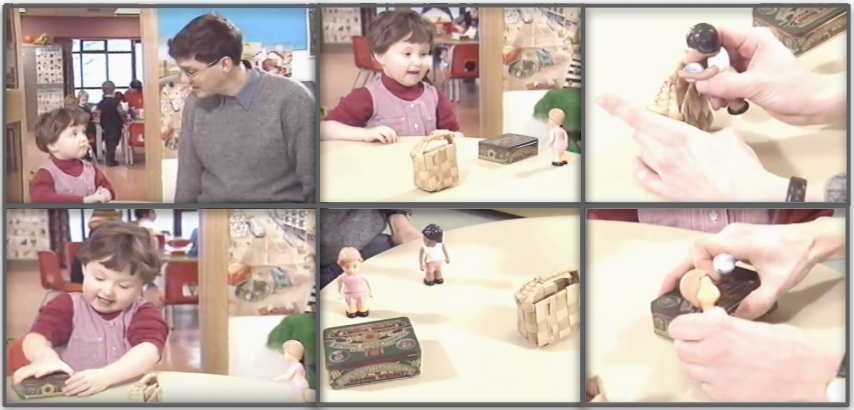
\includegraphics[width=1\linewidth]{./images-posterlatinr/tom-process3}
\\
\textbf{Figure 1:} Sally-Anne task
\end{center}
}


%%%%%%%%%%%%%%%%%%%%%%%%%%%%%%%%%%%%%%%%%%%%%%%%%%%%%%%%%%%%%%%%%%%%%%%%%%%%%%
  \headerbox{References}{name=references,column=0,above=bottom}{
%%%%%%%%%%%%%%%%%%%%%%%%%%%%%%%%%%%%%%%%%%%%%%%%%%%%%%%%%%%%%%%%%%%%%%%%%%%%%%
    \smaller
    \bibliographystyle{ieee}
    \renewcommand{\section}[2]{\vskip 0.05em}
      \begin{thebibliography}{1}\itemsep=-0.01em
      \setlength{\baselineskip}{0.4em}

\bibitem{curtis} Curtis, S. M. (2010). BUGS code for item response theory. \textit{Journal of Statistical Software}, 36:1-34.
\bibitem{revelle} Revelle, W. (2015). The psych package Version 1.5.8. URL \href{https://cran.r-project.org/web/packages/psych/psych.pdf}
\bibitem{sturtz} Sturtz, S., Ligges, U., and Gelman, A. (2005). R2WinBUGS: A Package for Running WinBUGS from R. \textit{Journal of Statistical Software}, 12(3):1-16. URL\href{https://www.jstatsoft.org/article/view/v012i03} 


      \end{thebibliography}
   \vspace{0.05em}
  }


%%%%%%%%%%%%%%%%%%%%%%%%%%%%%%%%%%%%%%%%%%%%%%%%%%%%%%%%%%%%%%%%%%%%%%%%%%%%%%
  \headerbox{Overview}{name=method,column=0,below=problem, above=references}{
%%%%%%%%%%%%%%%%%%%%%%%%%%%%%%%%%%%%%%%%%%%%%%%%%%%%%%%%%%%%%%%%%%%%%%%%%%%%%%

\begin{tcolorbox}
\textbf{{\large 1. Aim}}
\end{tcolorbox}
\noindent Understanding of mental states in children over the third year of life, that is over a year before they are supposed to pass belief
tasks, through MIRT.
\vspace{0.5em}
\begin{tcolorbox}
\textbf{{\large 2. Data Description}}
\end{tcolorbox}
\vspace{-1em}
\begin{center}
\textbf{Participants} 
\end{center}
\vspace{-0.5em}
86 British children (Female = 41, Male = 45) from different preschools and day nurseries located in Northern Lancashire. Age: Between 30 and 33 months when recruited.
\vspace{-1em}
\begin{center}
\textbf{Measures} 
\end{center}
\vspace{-0.5em}
8 mental state tasks (13 questions three times in intervals of 4 months). A correct response scored `1' and an incorrect response scored `0'.
\vspace{-0.5em}
\begin{table}[H]
\centering
\scalebox{0.91}{
\begin{tabular}{ll}
$\bullet$ Standard Location Change & $\bullet$ Pretense, Desire and Think\\ 
$\bullet$ Deceptive Box & $\bullet$ Verbal and Non Verbal\\
$\bullet$ Narrative & (2 and 4 trials respectively)  
\end{tabular}}
\end{table}

\vspace{-1em}
\begin{tcolorbox}
\textbf{{\large 3. Non-Longitudinal Analysis}}
\end{tcolorbox}
\vspace{-2em}
\begin{center}
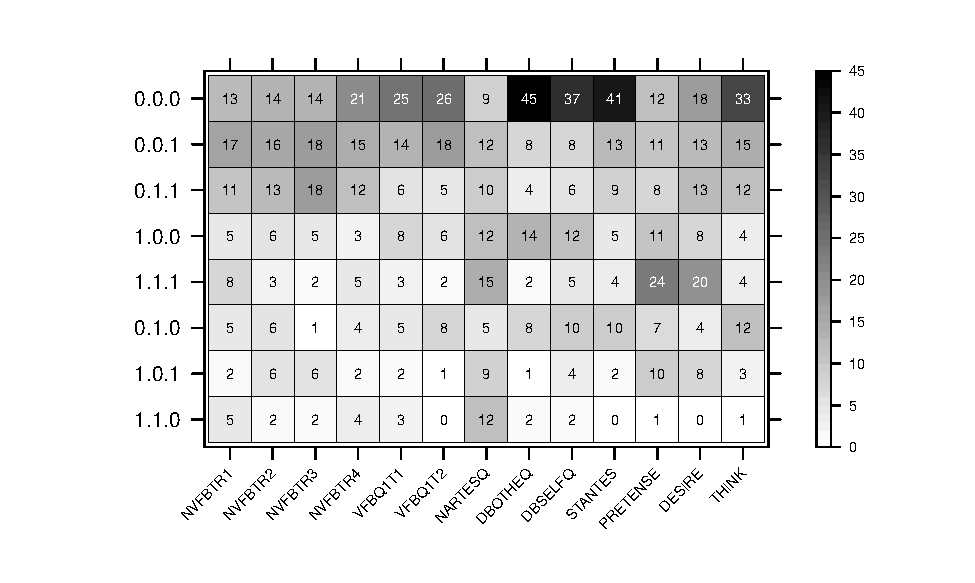
\includegraphics[trim=2cm 0.8cm 1.5cm 0.5cm,clip,width=1\linewidth]{./images-posterlatinr/Patterns}\\
\vspace{-0.4em}
\textbf{Figure 2:} Response Patterns
%\caption{Response Patterns}
\end{center}
\vspace{-1.4em}
\begin{center}
%\textbf{Figura 2:} \textbf{Left:} Response Patterns
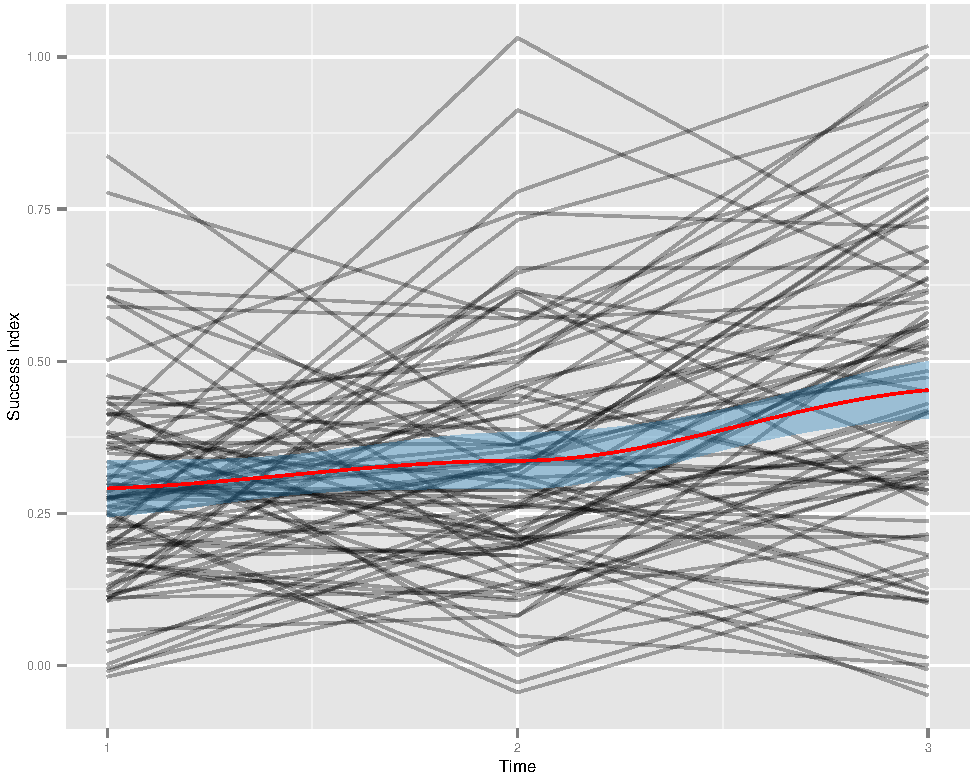
\includegraphics[width=0.8\linewidth]{./images-posterlatinr/IndexPerformance} \\
\vspace{-0.5em}
\textbf{Figure 3:} Total performance across time
\end{center}

%\begin{itemize}
%%\item Only complete observations taken into account
%\item \textbf{Top:} Most difficult tasks are Standard Location Change and Deceptive Box.
%\item \textbf{Bottom:} General trend is increasing.
%\end{itemize}

}



%%%%%%%%%%%%%%%%%%%%%%%%%%%%%%%%%%%%%%%%%%%%%%%%%%%%%%%%%%%%%%%%%%%%%%%%%%%%%%
\headerbox{Multidimensional Item Response Theory (MIRT)}{name=results,column=1,span=2,row=0}{
%%%%%%%%%%%%%%%%%%%%%%%%%%%%%%%%%%%%%%%%%%%%%%%%%%%%%%%%%%%%%%%%%%%%%%%%%%%%%%

\begin{multicols}{2}

\begin{center}
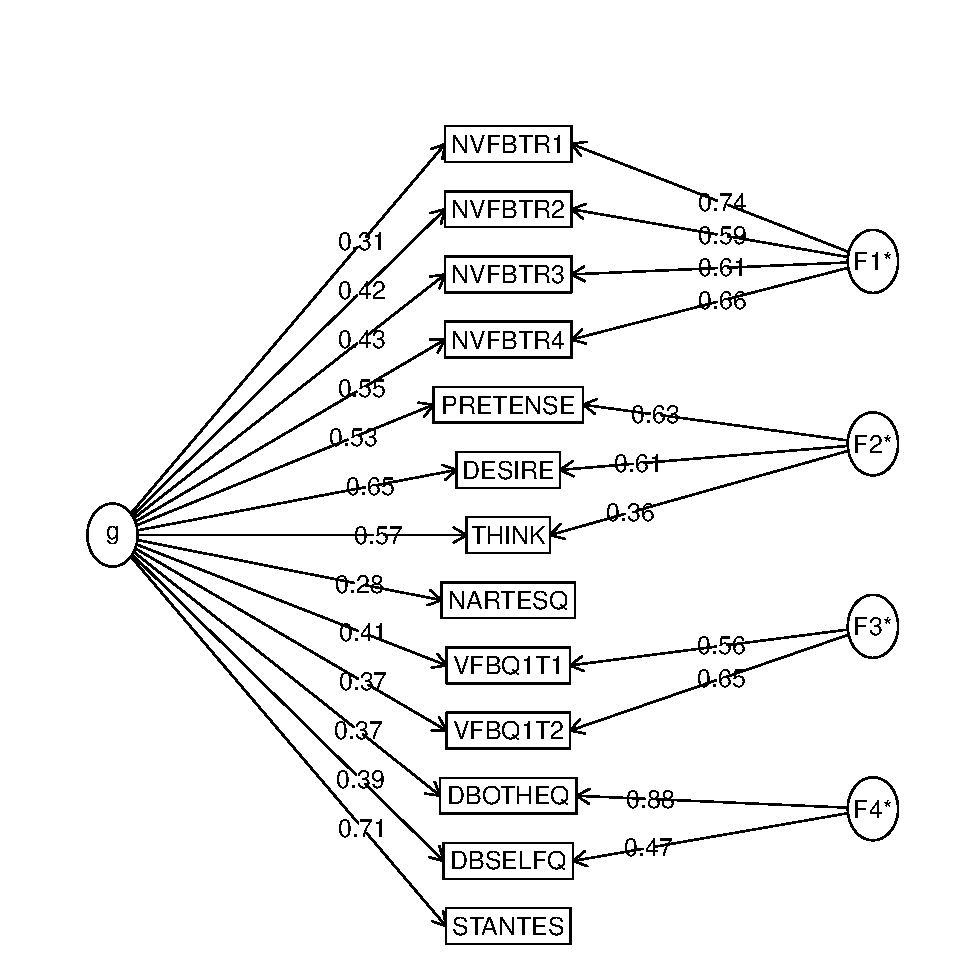
\includegraphics[trim=0 0 0 2cm,clip,width=1\linewidth]{./images-posterlatinr/BifactorPath} \\
\textbf{Figure 4:} Bifactor model Path. Use of \texttt{psych} package to do the structure, but not the output numbers.
\end{center}

\columnbreak

\begin{enumerate}
\item \textbf{Exploratory Factor Analysis}
\begin{itemize}
\item Not previous knowledge of the number of dimensions that comprises
ToM.
\item Dimensions estimated by comparing nested models.
\end{itemize}
\item \textbf{Confirmatory Factor Analysis}
\begin{tcolorbox}[title=Bifactor model]
A single factor is present in all the items, but with additional clusters
of local dependencies formed by other independent specific factors.
\end{tcolorbox}
\end{enumerate}

\vspace{-4em}
{\LARGE \[
\Downarrow
\]}
\centering
\textbf{Main Findings} 
\begin{itemize}
\item Dimensional reduction of ToM general ability.
\vspace{-0.5em}
\item ToM is comprised by 6 latent dimensions.
\end{itemize}

\end{multicols}

}

%%%%%%%%%%%%%%%%%%%%%%%%%%%%%%%%%%%%%%%%%%%%%%%%%%%%%%%%%%%%%%%%%%%%%%%%%%%%%%
  \headerbox{Conclusions}{name=background model,column=1, span=2, above=bottom}{
%%%%%%%%%%%%%%%%%%%%%%%%%%%%%%%%%%%%%%%%%%%%%%%%%%%%%%%%%%%%%%%%%%%%%%%%%%%%%%

\begin{enumerate}
\itemsep0em
\item Children before 4 years old successfully passed Pretense, Desire and NVFB tasks.
\item ToM reduced to \textbf{6 latent abilities} through the Bifactor Model.
\item \textbf{Easy items:} Pretense and Desire. \textbf{Most difficult item:} Standard Location Change.
\item Significant improvement across time: NVFB ability.
\item \textbf{Causal analysis:} Pretense, Desire and Think affects the development of most of the others abilities.
\end{enumerate}

}

%%%%%%%%%%%%%%%%%%%%%%%%%%%%%%%%%%%%%%%%%%%%%%%%%%%%%%%%%%%%%%%%%%%%%%%%%%%%%%
  \headerbox{The Two Stage Approach to determine Causality}{name=prueba,column=1, span=2, below=results,above=background model}{
%%%%%%%%%%%%%%%%%%%%%%%%%%%%%%%%%%%%%%%%%%%%%%%%%%%%%%%%%%%%%%%%%%%%%%%%%%%%%%

\begin{tcolorbox}
\textbf{{\large First Stage: Bayesian Longitudinal Analysis}}
\end{tcolorbox}
\vspace{-1em}
\begin{multicols}{2}
\centering
\textbf{Features of Modelling} \\
\vspace{0.3em}
\begin{itemize}
\item {\textbf{\underline{Correlation Structure}:}} Latent abilities on the same subject will be more correlated than among different subjects. 
%Autoregressive AR(1), Unstructured Covariance and Random Effects.
\vspace{-0.5em}
	\begin{itemize}
	{\item Autoregressive AR(1)}
	{\item Unstructured Covariance}
	{\item Random Effects}
	\end{itemize}
\item 3 chains of $10000$ iterations with a burn-in phase of $5000$ and final results pooled in a single chain.
\item Employment of a \textbf{BUGS} (\textbf{B}ayesian inference \textbf{U}sing \textbf{G}ibbs \textbf{S}ampling) code called from the free software \textsf{R}.
\end{itemize}

%\vspace{1em}

\begin{center}
\textbf{Model Selection} 
\vspace{-1em}
%{Summary of DIC criterion}
%\vspace{-0.5em}
\begin{table}[H]
\centering
\caption{Summary of DIC criterion}
\scalebox{0.93}{
\begin{tabular}{lccc}
\hline
\textbf{Model} & $\text{DIC}$ & $\boldsymbol{\text{Q}_{0.025}}$ & $\boldsymbol{\text{Q}_{0.975}}$ \\ 
\hline \hline
AR(1) Covariance Structure & \color{blue} 2312.46 & 2205.88 & 2418.96 \\ 
Unstructured Covariance & \color{red} 2242.62 & 2124.69 & 2359.80 \\ 
Random Effects & 2337.56 & 2258.15 & 2415.93 \\ 
\hline
\end{tabular}}
\label{table_dic}
\end{table}
\end{center}

\begin{itemize}
\item Smaller values of DIC suggests a better model.
\vspace{-0.5em}
\item Final Model: AR(1) Covariance Structure
\end{itemize}

\columnbreak

\textbf{Estimation Results} 
\vspace{-1em}
\begin{table}[H]
\centering
\caption{Summary of $\rho$ estimate}
\scalebox{0.8}{
\begin{tabular}{lccc}
\hline
\textbf{Factor} & $\boldsymbol{\bar{\rho}_f}$ & $\boldsymbol{\text{Q}_{0.025}}$ & $\boldsymbol{\text{Q}_{0.975}}$ \\ 
\hline \hline
Non Verbal FB & 0.44 & 0.22 & 0.63 \\ 
Pretense, Desire, Think & 0.65 & 0.43 & 0.83 \\ 
Verbal FB & 0.37 & 0.00 & 0.74 \\ 
Deceptive Box & 0.47 & 0.08 & 0.84 \\ 
Narrative & 0.06 & -0.86 & 0.88 \\ 
Location Change & 0.62 & -0.16 & 0.98 \\
\hline
\end{tabular}}
\label{table_rho}
\end{table}
\vspace{-2em}
\begin{center}
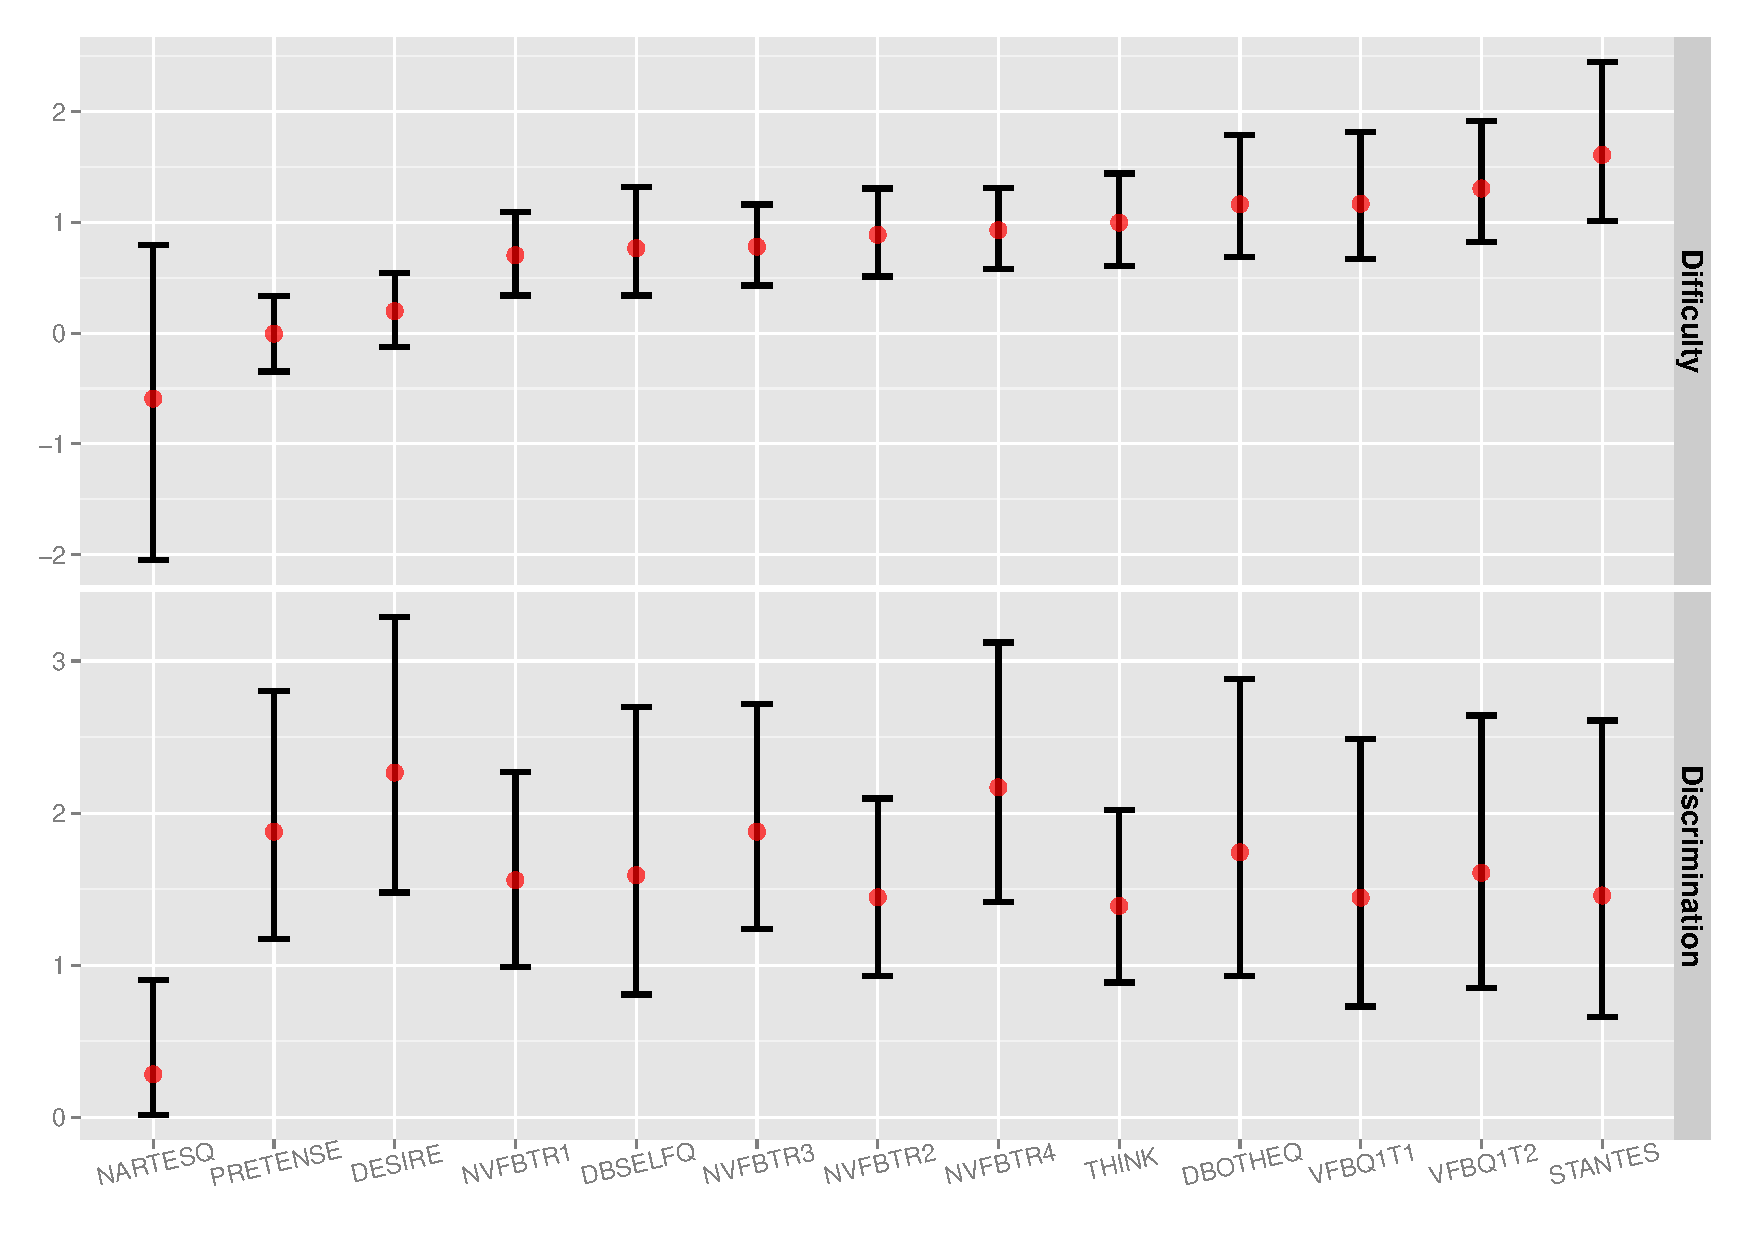
\includegraphics[trim=0cm 0.5cm 0cm 1cm,clip,scale=0.3]{./images-posterlatinr/diff_disc_AR1}
\textbf{Figure 5:} Credibility Interval of Item parameters considering AR(1) as covariance structure.
\end{center}

\end{multicols}

\vspace{-0.5em}
\begin{tcolorbox}
\textbf{{\large Second Stage: Ability Regression}}
\end{tcolorbox}
Regression of the latent ability factors of $t=2,3$ against the latent ability of the previous instant of times.
\vspace{-0.5em}

%\begin{multicols}{2}
%\begin{center}
%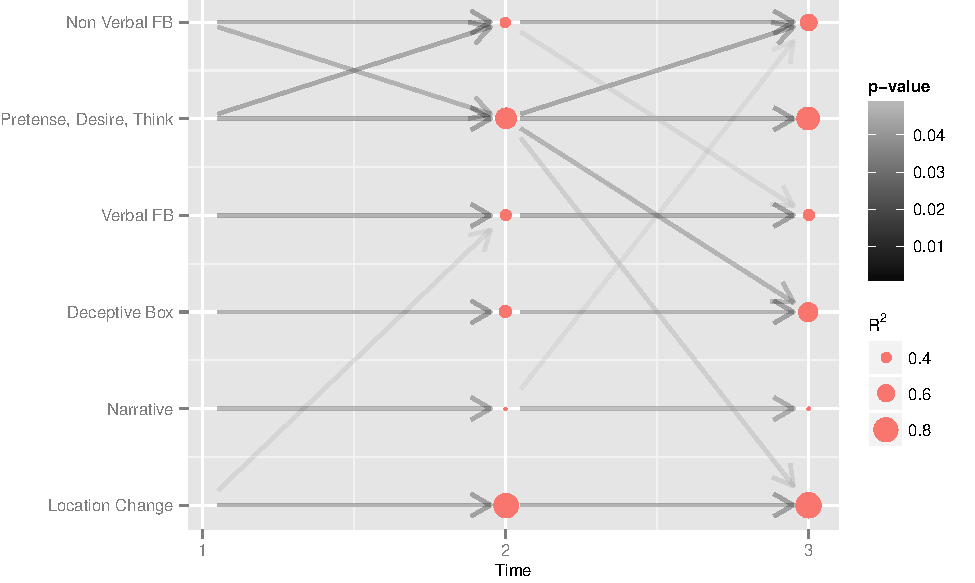
\includegraphics[scale=0.7]{./images-posterlatinr/causal_AR1}
%\end{center}
%\vspace{-1em}
%\textbf{Figure 6:} Path Diagram of Causality - Model AR(1). The p-values have not been adjusted for multiple comparison.
%
%\columnbreak
%
%\end{multicols}

\begin{figure}[H]
\centering
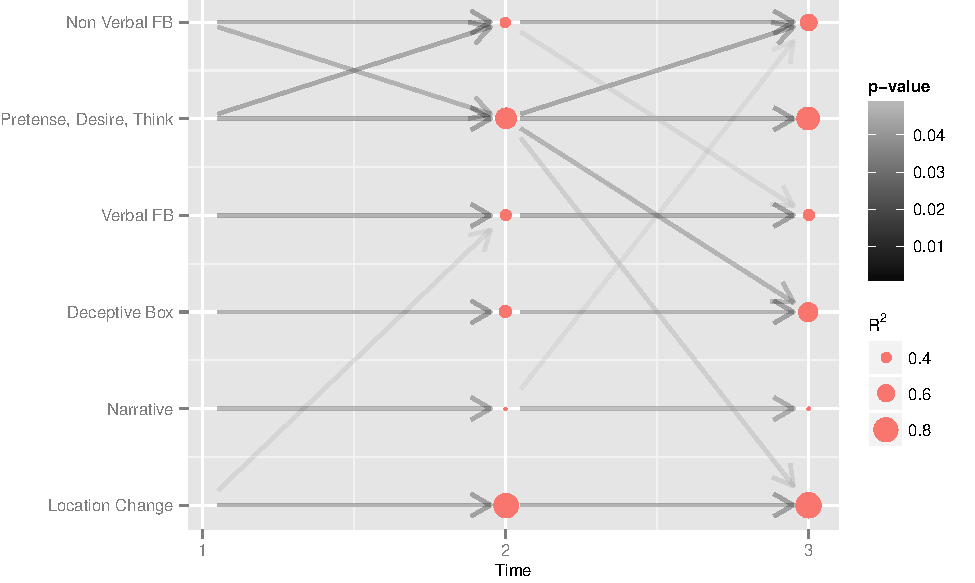
\includegraphics[scale=0.7]{./images-posterlatinr/causal_AR1}\\
\textbf{Figure 6:} Path Diagram of Causality - Model AR(1). \\
The p-values have not been adjusted for multiple comparison.
\end{figure}

}

\end{poster}

\end{document}

